\section{モノを分解する}

最初の仕事は、問題からその問題を解決するための大まかなアーキテクチャに至るまで、どのようにすればよいかを考えることです。第6章「コンポーネントの作成」で説明したように、問題を分析し、個別のコンポーネントを特定します。アプリケーション内 (あるいは複数のアプリケーションにまたがる) で汎用的なコンポーネントを再利用したり、チーム内で開発を分担したり、あるいは一度に問題の一部だけを考えることができるような構造にしたりするためです。

コンポーネントを分離する方法にルールはありませんが、いくつかの一般的なガイドラインに従うことは可能です。コードをグループ化する理由としては、関数が同じ種類のデータで動作する、データの範囲や寿命が共通である、外部要件による変更の可能性が似ている、必要なリソースが似ている、などがあります。もし、あるコードのセットが、複数のコンテキストで異なる設定をしたときに再利用可能であれば、それは間違いなく有用なコンポーネントである。

この議論を具体化するために、次のような問題を考えてみよう。私たちの会社は、ソーシャルメディア上の製品に関する言及を監視し、それに対応できるシステムを必要としています。その応答は、タイムリーで、有用で、適切であることが重要である。この役割を果たす人はいますが、当社の製品は非常に人気があるため、注意が必要なメッセージを見つけ、回答候補を作成し、その回答を送信するというプロセスを自動化するための支援が必要です。

この問題を考えているうちに、アプリケーションにいくつかの境界線が見えてきました。ソーシャルメディアフィードの監視を自動化する場合、各サードパーティシステムとのやり取りをカプセル化するコンポーネントが必要です。これらのフィードは、個々のシステムとのやり取りは別々であっても、それ自体は多くの類似した実装ニーズを共有することができます。フィードは、外部リソースを使用し、そのライフサイクルをフィードに結合しているため、別個のコンポーネントとなります。

同様に、メッセージにどのように応答するかというルールの知識ベースをカプセル化するコンポーネントが必要になります。これは自己完結型でも、外部システムを使ってルールを呼び出すことも可能です。

最後に、元のメッセージと応答候補を受け取り、それらをソーシャルメディアの専門家に提示して、メッセージを承認するか修正するかを決定するコンポーネントが必要になると思われます。このコンポーネントは、ある人物へのアクセスを処理する役割を担っています。

アーキテクチャとそのハイレベルなコンポーネントがどのようなものかは、スケッチでご覧いただけます。 

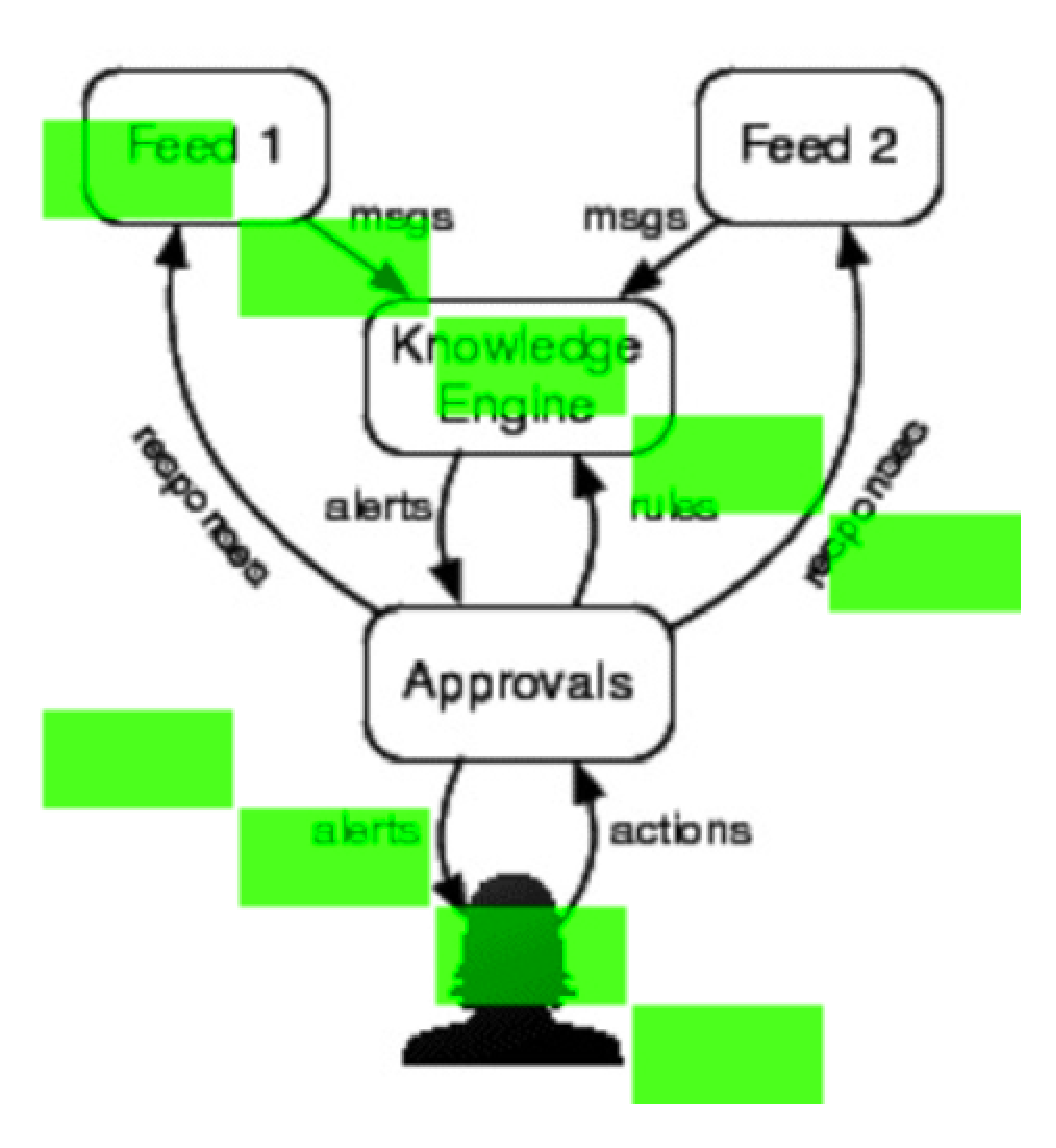
\includegraphics[width=8cm]{fig_07_001.eps}

次に、必要となるコンポーネントを定義し、それらをどのように接続するかを考えてみましょう。システムを組み立てていく上で、アプリケーションやコンポーネントのライフサイクルを考慮する必要がある。Clojureでこのような問題に最適なライブラリはComponentです\[20\]。コンポーネントを定義しながら、Componentを介してライフサイクルの開始と停止の機能を設定します。









